% !TEX root = Thesis.tex
\chapter{Introduction}\label{chap:Intro}

  In the late nanoscale CMOS era, automated layout generation of advanced technologies has drawn more attention due to the growing demand in industry. As the complexity of the advanced nodes for analog circuit increases, the layout constraints and the expanding performance requirements become major productivity bottlenecks. Lately, in order to alleviate the impact from process variation beyond the transistor level as well as striving for excellent performance, analog layout design mostly relies on designers' expertise. However, the iterative refinement on manual design damages the productivity of analog layout. Therefore, it is more efficient to enroll the know-how from existing designs instead of generating a new one. To migrate layout template via preservation becomes a plus.

  For analog layout, reusability relies on the similarity such that part of source layout can be reused to add new modules or layers on target layout with minor modification. To preserve the design knowledge from the template layouts, the devices' relative positions and the routing behaviors should be considered thoroughly. Typical analog constraints such as symmetry and proximity constraints fundamentally regulate the placement. On the other hand, wire symmetry and topological matching are critical to analog routing. Placement and routing extracted from the template layout can benefit layout migration. In other words, more informations are extracted from template layout, more circuit characteristics are preserved. Currently, analog layout preservation pays more attention on placement~\cite{cart-hammouda-dac06,cbc-bhattacharya-dac04,Wang_ALRGP_TODAES2011} 
  for topology extraction. However, seldom do we study routing behavior extraction in previous works. In all, a solution to preserve the correlation during layout retargeting, or so-called layout migration is critical.


  \begin{figure}
    \centering
    \begin{subfigure}[t]{0.4\textwidth}
    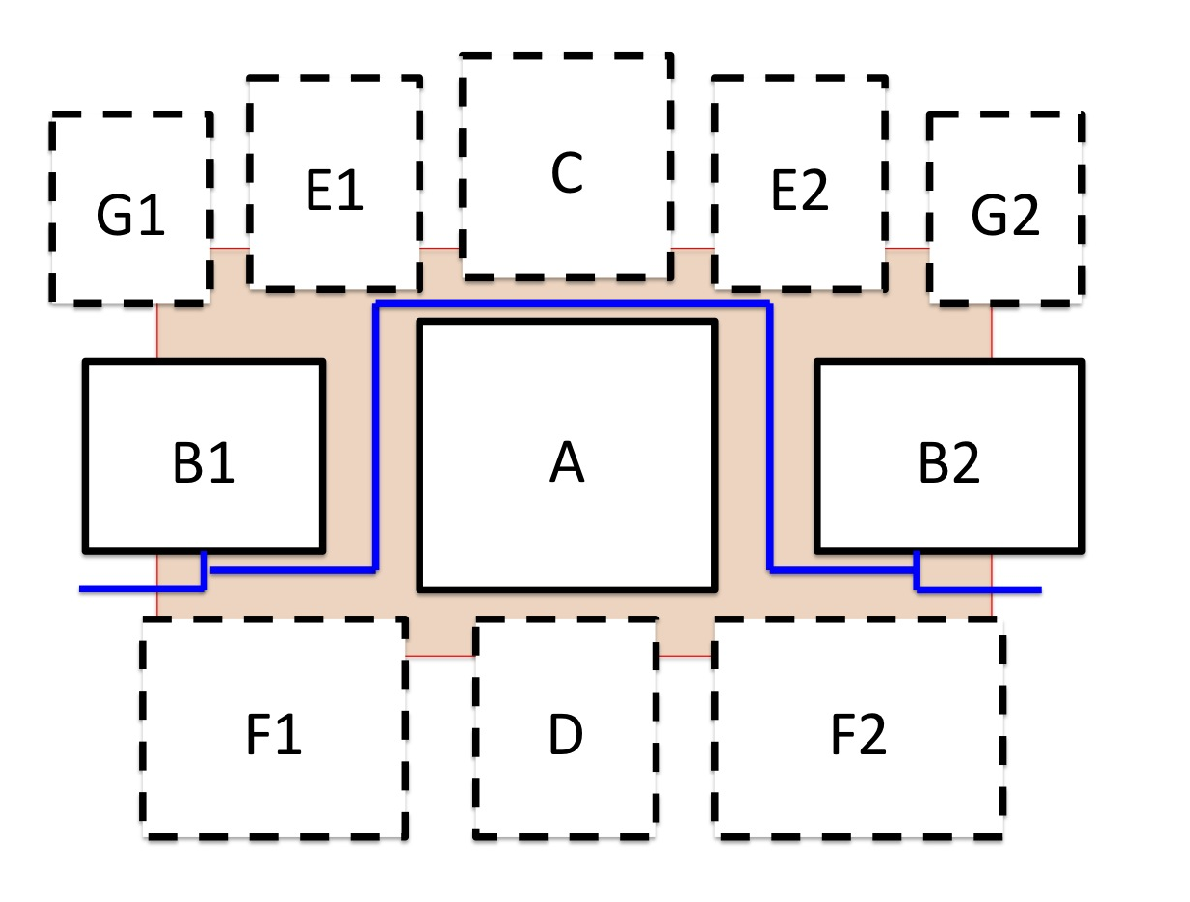
\includegraphics[width=\textwidth]{Fig/RoutingPreserv_a.eps}
    \caption{Reference template layout}
    \label{fig:RoutingPreserv_A}
    \end{subfigure}
    \begin{subfigure}[t]{0.4\textwidth}
    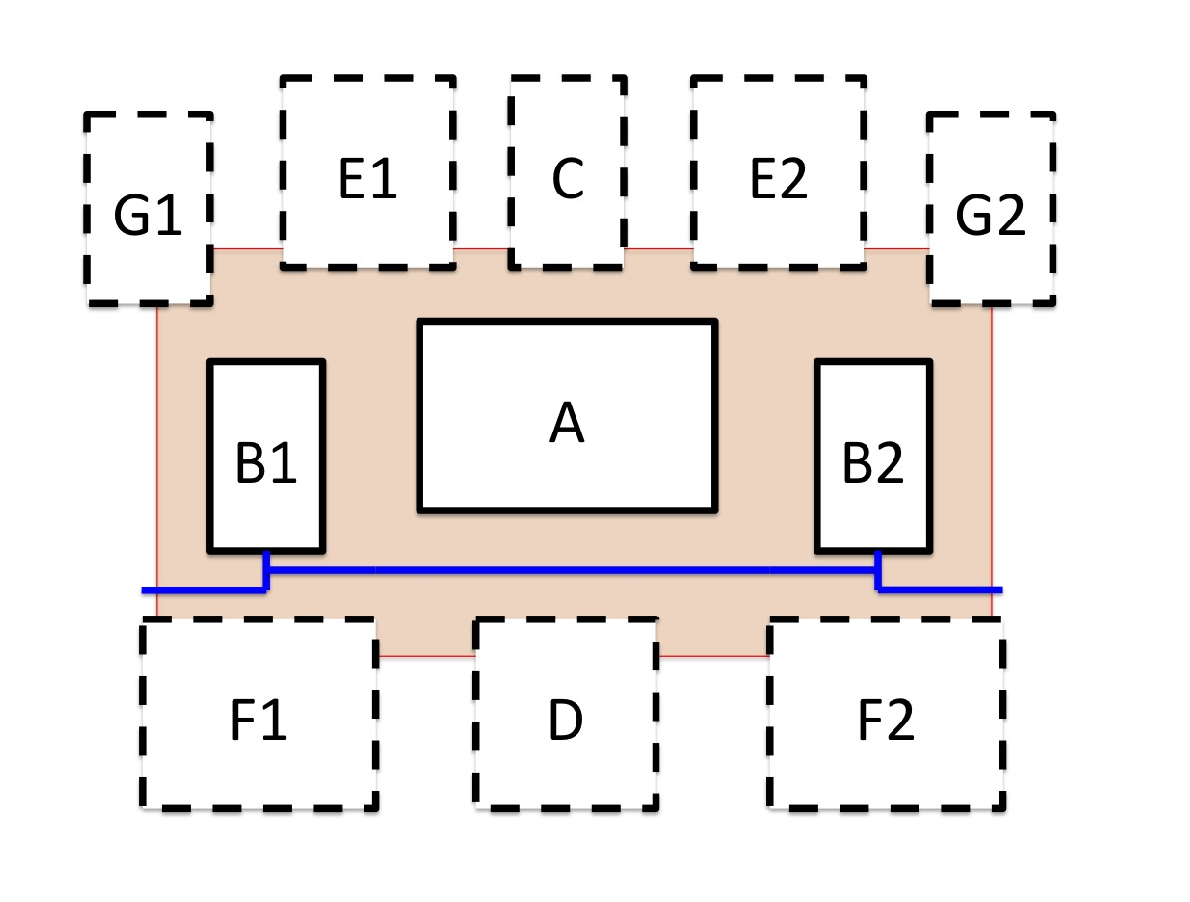
\includegraphics[width=\textwidth]{Fig/RoutingPreserv_b.eps}
    \caption{Non-preserved automatic routing}
    \label{fig:RoutingPreserv_B}
    \end{subfigure}
    \begin{subfigure}[t]{0.4\textwidth}
    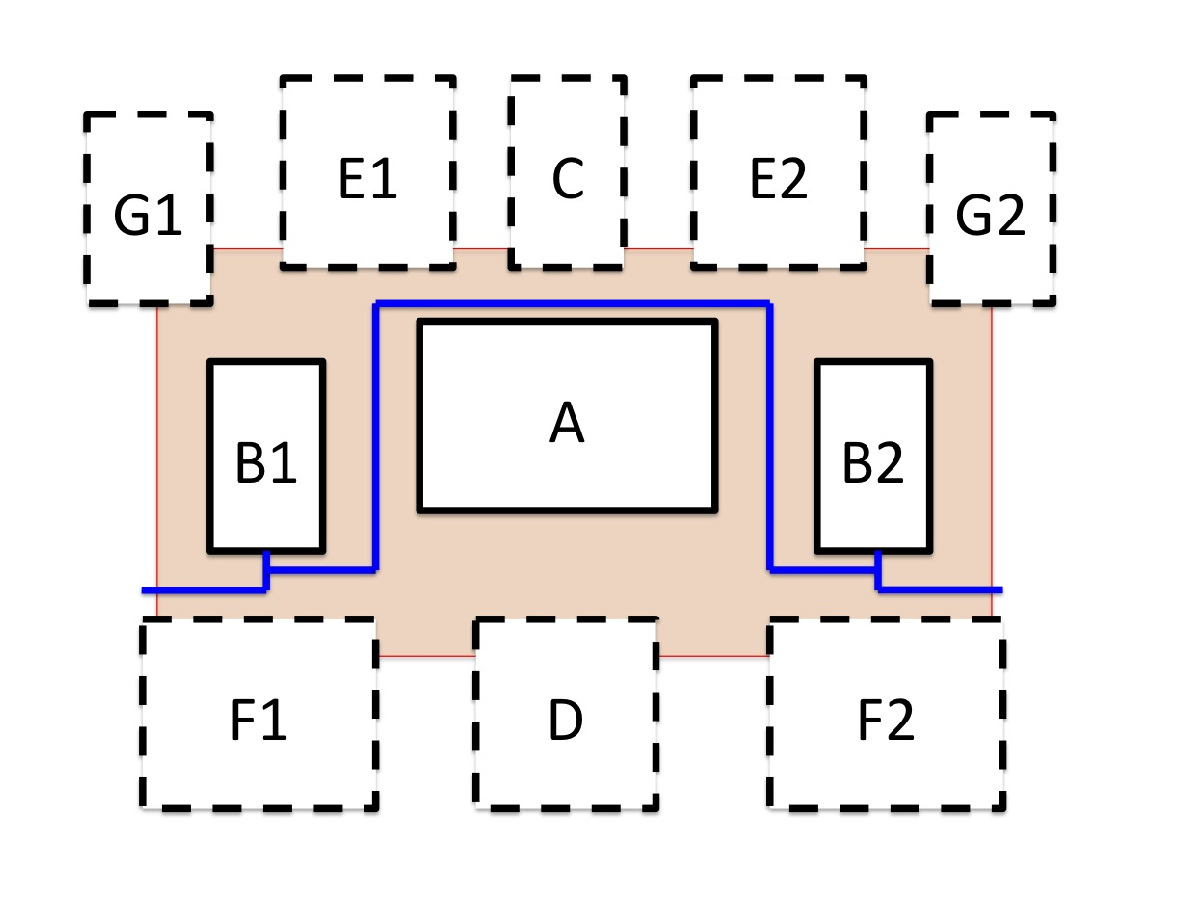
\includegraphics[width=\textwidth]{Fig/RoutingPreserv_c.eps}
    \caption{Preserved routing}
    \label{fig:RoutingPreserv_C}
    \end{subfigure}
    \begin{subfigure}[t]{0.4\textwidth}
    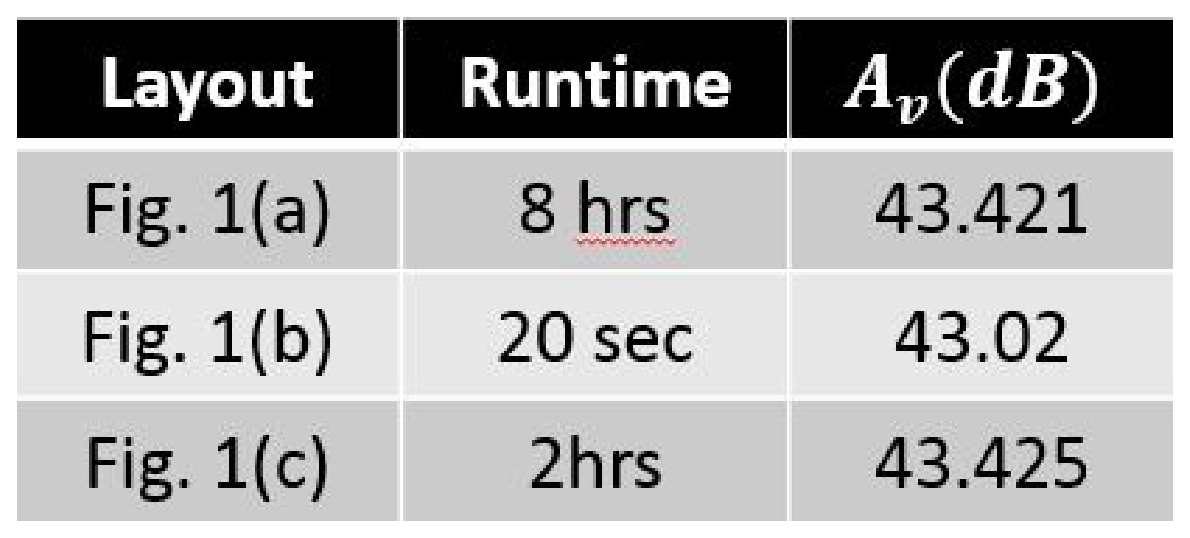
\includegraphics[width=\textwidth]{Fig/RoutingPreserv_d.eps}
    \caption{Timing and simulation results}
    \label{fig:RoutingPreserv_d}
    \end{subfigure}
    \caption{Analog layout generation with different configuration. (a) Reference layout with complete placement and routing. (b) non-preserved automatic routing considering usual constraints only. (c) layout generation considering preserved routing characteristics. (d) simulation results in umc65nm technology.}
    \label{fig:RoutingPreserv}
  \end{figure}

  A simple experiment shows the necessity of routing preservation. In Fig.~\ref{fig:RoutingPreserv}, we compare the analog layout generation with two configurations. Fig.~\ref{fig:RoutingPreserv_B} automatically generates analog layout with respect to analog constraints only, and Fig.~\ref{fig:RoutingPreserv_C} keeps more preserved routing informations from the reference layout in Fig.~\ref{fig:RoutingPreserv_A}. Even though the routing path in Fig.~\ref{fig:RoutingPreserv_C} from $B1$ to $B2$ is detoured in the reference layout, the simulation result obviously shows that it earns better performance than Fig.~\ref{fig:RoutingPreserv_B} on voltage gain over 0.4$dB$, which makes the path straightly connecting across the tunnel between $A$ and $D$. Under the same configuration of circuit sizing, these two layouts represent the performance response of reusability. According to the original perspective of design, the detour benefits the parasitic effect of the intersection on wires. Besides the performance result, we also observe that the runtime of Fig.~\ref{fig:RoutingPreserv_C} is remarkably improved than Fig.~\ref{fig:RoutingPreserv_B}. 
  
  There are more layout generation experiments illustrated in Section~\ref{sec:Exp}, and these experiments show that automatically generated layouts with preserved information have superior performance. Meanwhile, the preserved information represents the routing behavior extracted from the original layout. By applying the preserved routing behavior, it can produce the migrated layout more efficiently than manually migration. As a result, migration with preserved information facilitates the flow of layout generation, that reduces the time-to-market. In other words, the productivity is raised.

  \section{Previous Works}\label{sec:PreWork}

  The problem of layout retargeting has been widely discussed in the literature. We can roughly categorize them into two major stages, placement and routing. At the placement stage, certain approaches mainly focus on fully mapping~\cite{Bhattacharya_ASPDAC04,cbc-bhattacharya-dac04,msc-bhattacharya-tcad06,Zhang_TCAD08,LayoutRetarg_Liu_ASPDAC2010,Wang_ALRGP_TODAES2011}. First of all, Bhattacharya et al. in~\cite{Bhattacharya_ASPDAC04} detect the symmetric components from the source layout hierarchically and retarget it. \cite{cbc-bhattacharya-dac04} later enhance the retargeting layout with compaction. Hammouda et al. in\cite{cart-hammouda-dac06} combine the device resizing, layout compaction as a full layout retargeting flow. In \cite{msc-bhattacharya-tcad06}, Bhattacharya et al. extend the compaction to larger analog design as the multi-level layout generation. Moreover, in \cite{Zhang_TCAD08}, Zhang et al. deal with the parasitic effects as well as retargeting the compaction-based layout. Wang et al. build template for analog layouts and then use geometric programming to guarantee the global optimal solution for compaction in \cite{Wang_ALRGP_TODAES2011}. 

  Since compaction holds almost the same topology from the source layout, it constructs a symbolic structure to preserve layout topology, technology rules, symmetry and proximity constraints. Additionally, Weng et al. in~\cite{ALP_YPWeng_iccad2011} provide prototypes with Defer~\cite{defer_jackey_tcad10} in migrated layout due to the different scale ratio among devices efficiently. Method in~\cite{ALP_YPWeng_iccad2011} successfully reduces the white space under target technology and obtains better performance after post-layout simulation. 

  For routing, the existing researches rely more on routing generation with constraints rather than retargeting. Early works in~\cite{KOAN_ANAGRAMII-JSSC1991,aicon_malE_tcad96,ppraic_Linfu_iccad2010} propose a maze-style router in order to consider symmetry and non-symmetry modules in the same design. Channel routing is also adopted by~\cite{cbcrams_UChoudhury_tcad93} and \cite{aicon_malE_tcad96} to deal with mirror symmetry and detailed routing among blocks. Recently, other than symmetry issue, exact matching constraints for maze routing are well addressed in ~\cite{ermams_MMOzdal_tcad09}. Ou et al. in \cite{numarmc_HCOu_dac12} first define three typical matching constraints for analog routing which dominates performance most: {\it(1)symmetry, (2)topology-matching} and {\it (3)length-matching}. 

  Additionally, Pan et al. in \cite{Pan_CGR_ICCAD2012} claim that routing priority considering constraint group in hierarchy can enhance the signal integrity. Still, work in LAYGEN II \cite{LAYGENII_TCAD13} performs an evolutionary multi-objective way to evaluate an optimized routing results from layout templates. Lately, \cite{SAPR_DAC13} proposes a simultaneous analog placement and routing framework which further considers the current flow constraints for critical nets. Overall, although the symmetry and matching constraints are well treated and routing matching constraints are extended further, the correlation among wires and placement has not been systematically preserved as a guideline to migrate.

  \section{Our Contributions}\label{sec:contribution}

  While the aforementioned mechanisms successfully facilitate layout migration with designers' know-how on placement, the behavior of routing has not been extracted essentially. Thus, the template-based layout migration does not benefit routing much. 
 
  In addition, the routing generation relies on automatic routing methodologies with respect to the placement constraints. Such constraints in ~\cite{cbc-bhattacharya-dac04,Bhattacharya_ASPDAC04,msc-bhattacharya-tcad06,Zhang_TCAD08,Wang_ALRGP_TODAES2011} are not suitable for routing generation. 

  In this paper, we propose an analog layout migration flow with the best preservation that rapidly generates the analog layout on the target technology. We briefly sum up our contributions as follows:

  \begin{itemize}
    \item {\bf A layout extraction mechanism with placement and routing behavior} is proposed. Layout extraction requires not only topology of device modules, but also the relationship among wires and design blocks. Aside from utilizing the method in \cite{ALP_YPWeng_iccad2011} to extract the blocks, a routing preservation algorithm is followed by in this work. Such preservation algorithm via Constrained Delaunay Triangulation (CDT)~\cite{Shewchuk200221} decomposes the modules and routing channels with a set of triangles.  
    \item {\bf A bottom-up prototyping framework for analog layout migration} is delivered. According to the information extracted from the existing layout, the full layout with placement and routing can be migrated automatically with high reusability. This multilevel framework simultaneously reduces the redundancy of routing as well as achieving the qualified circuit performance.
    \item {\bf A wire refinement methodology} is proposed to further improve performance metrics right after the routing settled. Given the target technology design rules, placement, wires and pin connection information, it is sufficient to explore the optimization of the width of wires.
    \item {\bf A fast multiple analog layout generator} illustrates that our prototyping framework is capable of producing routing results with different topologies from the source layout. The resultant layouts show that our representation realizes multiple layouts efficiently.
  \end{itemize}

  Current layout migrations limit the flexibility of routing reconstruction. This work achieves effective and adjustable layout retargeting. Yet, it allows designers to decide the relevant solution from multiple candidates. Some of previous results were presented in \cite{Chin_DMR_ICCAD2013}. Instead, this work appreciates the comparison with state-of-the-art.

  The rest of this paper is organized as follows. 
  Chapter~\ref{chap:prelim} first reviews the definition of PSLG and CDT, and then states the analog layout migration problems. 
  Chapter~\ref{chap:migration} describes the full layout migration framework and its dominance.
  Chapter~\ref{chap:LayoutExtPre} presents the extracting and preserving techniques for placement and routing. 
  Chapter~\ref{chap:prototyping} describes the layout prototyping with placement and routing generation. In the end of our proposed framework, Chapter~\ref{chap:WireSegRefine} delivers a methodology to refine the width of wires in order to explore better performance. 
  We demonstrate the experimental results in Chapter \ref{chap:Exp}, and Chapter~\ref{chap:Conclusion} concludes this paper. 
